\subsection{Conditional proposals and observation-weighted parents}
\label{sec:observation-weighted-default}
The observation can improve a proposal in two distinct places. It can change
where a child is drawn conditional on a particular physical parent, and it can
change which parent receives that child. The UKF moments and the LEDH flow
already use the observation to modify continuous proposal geometry. They do
not, by themselves, replace a uniform allocation over physical parents by
allocation proportional to those parents' predictive observation probabilities.
This distinction explains why observation-weighted selection adds something
even when the previous proposal was observation-informed.

For the SIR model considered here, the transition mean is nonlinear but the
transition noise is additive Gaussian and the observation is linear Gaussian.
Condition on the equal-weight incoming cloud $x_{t-1}^{1:N}$ after reset and
write $a_i=f_\theta(x_{t-1}^i)$. Its predictive mixture is
\begin{equation}
 p_N(x)=\frac1N\sum_{i=1}^N\varphi(x;a_i,Q),\qquad
 g(y\mid x)=\varphi(y;Hx,R).
\end{equation}
Each component can therefore be conditioned exactly, without replacing the
nonlinear transition by a globally linear transition. Define
\begin{align}
 S&=HQH^\top+R,& K&=QH^\top S^{-1},\\
 e_i&=\varphi(y;Ha_i,S),&
 c_i&=a_i+K(y-Ha_i),& C&=Q-KSK^\top,\\
 Z_N(y)&=\frac1N\sum_i e_i,&
 \alpha_i&=\frac{e_i}{\sum_j e_j}.
\end{align}
Here $e_i$ measures how well the observation is predicted by parent $i$,
$c_i$ is that parent's observation-conditioned child mean, and $C$ is its
conditional covariance. In computation the equivalent Joseph expression
$C=(I-KH)Q(I-KH)^\top+KRK^\top$ avoids subtracting two nearly equal matrices.
The implementation propagates the derivatives of $Q,R,H,a_i,K,C$ and $Z_N$.

Uniform parent selection gives
$q_{\rm cu}(x)=N^{-1}\sum_i\varphi(x;c_i,C)$. Observation-weighted parent
selection instead gives
\begin{equation}
 q_{\rm cw}(x)=\sum_i\alpha_i\varphi(x;c_i,C)
             =\frac{g(y\mid x)p_N(x)}{Z_N(y)}.
 \label{eq:observation-weighted-bayes-identity}
\end{equation}
The last equality follows component by component from Gaussian conditioning,
then summing $g(y\mid x)\varphi(x;a_i,Q)=e_i\varphi(x;c_i,C)$ over $i$.
It both establishes the sampling law and provides an efficient marginal
proposal density. Merely changing the parent draw while retaining the old
uniform-mixture denominator would be wrong.

The new default replaces the global proposal branch by $q_{\rm cw}$ while
retaining the defensive identity and local-flow branches. With their declared
probabilities $\beta_0,\beta_1,\beta_2$, the actual proposal and weight are
\begin{equation}
 q_{\rm mix}(x)=\beta_0 p_N(x)+\beta_1 q_{\rm cw}(x)
                       +\beta_2 q_{\rm local}(x),\qquad
 \widetilde w(x)=\frac{g(y\mid x)p_N(x)}{q_{\rm mix}(x)}.
\end{equation}
Thus every branch retains the same target numerator and uses the density of
the full mixture. The original three-branch proposal and the intermediate
conditional proposal with uniform parents remain explicit comparison choices.
The conditional default is implemented once for affine Gaussian observations;
unsupported observation laws require an explicit alternative policy.

\subsection{What the ESS improvement establishes}
For normalized importance weights $W_i$, the effective sample size is
$\operatorname{ESS}=1/\sum_i W_i^2$. It equals $N$ for equal weights and
approaches one when a single child carries nearly all the mass. Increasing ESS
therefore reduces weight concentration within the represented cloud.
On the saved low-observation-noise SIR failure case (seed 1104, $N=1008$,
$T=2$), rerunning each complete filter from the same initial data gave the
following terminal effective sample sizes. Each filter has its own intervening
cloud, so this is an end-to-end comparison, not an insertion into an identical
second-step cloud.
\begin{center}
\begin{tabular}{lr}
\hline
Proposal & Terminal ESS\\\hline
Original three branches & 2.404\\
Conditional global branch, uniform parents & 6.495\\
Conditional global branch, observation-weighted parents & 392.512\\
Conditional-only, observation-weighted parents & 1008.000\\\hline
\end{tabular}
\end{center}
The weighted conditional mixture raises ESS by about $163$ times relative to
the original three branches in this case. This is a substantial reduction in
weight concentration and a useful robustness improvement. It does not imply
an equally large reduction in likelihood or score error.

Indeed, if the conditional-only proposal is used, equation
\eqref{eq:observation-weighted-bayes-identity} makes every importance weight
$Z_N(y)$, and ESS equals $N$ up to roundoff. That statement holds even if the
incoming cloud poorly approximates the filtering distribution. ESS measures
weight balance among the sampled children; it does not measure the accuracy
of the incoming mixture or the total likelihood derivative.

The first score comparison used eight paired streams at $T=10$, $N=1008$
and nominal SIR parameters. Componentwise RMSE relative to the saved,
approximate Zhao--Cui reference was
\begin{center}
\begin{tabular}{lrrr}
\hline
Proposal & Infection score & Recovery score & Noise score\\\hline
Original three branches & 1353.19 & 590.64 & 802.52\\
Conditional, uniform parents & 24.32 & 12.34 & 3.39\\
Conditional, weighted parents & 41.08 & 9.48 & 4.43\\\hline
\end{tabular}
\end{center}
All 24 streams passed their recorded validity checks. Conditioning the child
proposal was descriptively favorable in this experiment. The additional parent
weighting gave mixed score results: it reduced the recovery-score RMSE but
increased the other two relative to uniform conditional parents. With eight
streams, heavy tails and an uncertified reference, this table does not
establish a statistical ranking. The separate six-stream conditional-only
comparison likewise showed that ESS equal to $N$ does not guarantee the
smallest score error. The archived result is
\texttt{ledh-parent-selection-score-result-20261028.md}.

The owner-selected default on 28 October 2026 is consequently a proposal and
weight-concentration decision. It is not a claim that the score problem has
been solved. Analytical recursive differentiation includes the continuous
proposal, density and reset dependencies, but holds categorical parent indices
locally fixed. Agreement with finite differences away from switching boundaries
verifies that finite-program derivative; it does not establish a globally smooth
HMC target or equality to the exact model likelihood score. The new comparison
therefore evaluates likelihood and all score components separately at
$T=10,20,50$, using multiple SIR parameter points, paired streams, simple
proposal controls and two independently fitted Zhao--Cui references. Reference
importance overlap and disagreement between fits must be reported alongside
any accuracy conclusion.


\subsection{Likelihood and score comparison across SIR parameter points}
The expanded experiment holds the observations fixed and evaluates the same
likelihood at several parameter values. The three parameters are logarithms
of multiplicative changes in the infection rate, recovery rate and observation
noise scale. We use the first $10$, $20$ and $50$ observations from one saved
SIR dataset, with $N=1008$ particles and paired random streams across proposals.
Consequently, differences across parameter points describe a neighborhood of
this dataset's likelihood; they do not describe performance across independently
generated epidemics. The flow and reset controls are held fixed to isolate
proposal changes, rather than tuned separately to make each method competitive.
The calculation uses FP64 GPU/XLA as a precision comparison, not as evidence
that the production TF32 route is ready for admission.

The comparison uses two previously fitted Zhao--Cui adapted smoothers, following
the path-importance construction in \citet[eq.~(26), Algorithm~4]{zhao2024tensor}, with
ranks $20$ and $40$ and different fit seeds. Each supplies $M=100000$ complete
paths for each horizon. Let $\theta_0$ denote the parameter used to construct a
saved proposal $r$, and let $X^{(m)}$ denote its sampled path. At another
parameter $\theta$, retaining the same proposal gives
\begin{align}
 \ell_m(\theta)
 &=\ell_m(\theta_0)
   +\log p_\theta(X^{(m)},y_{1:T})
   -\log p_{\theta_0}(X^{(m)},y_{1:T}),\\
 \widehat L_r(\theta)&=\frac1M\sum_m\exp\{\ell_m(\theta)\},\\
 \widehat s_r(\theta)&=
 \sum_m\frac{\exp\{\ell_m(\theta)\}}
              {\sum_j\exp\{\ell_j(\theta)\}}
       \nabla_\theta\log p_\theta(X^{(m)},y_{1:T}).
\end{align}
Here $\ell_m(\theta_0)$ already contains the saved proposal denominator.
Thus the normalizer and score refer to the same importance calculation, and
$\widehat s_r=\nabla_\theta\log\widehat L_r$ when the saved proposal and paths
are held fixed. The analytical complete-data derivative is also checked against
independent canonical-model finite differences. This provides a useful
approximate reference; it does not turn a fitted tensor-train proposal into
an exact likelihood oracle.

Reference reliability changes sharply with the evaluation point. The
predeclared screening rule requires path ESS at least $1000$ out of $100000$
for both fits and agreement in the log likelihood and each score component
within three combined conditional jackknife standard errors. The nominal point
and noise multiplier $0.8$ pass at every horizon. Noise multiplier $1.25$ passes
at $T=20,50$ but fails at $T=10$, where one fit has path ESS about $425$.
Every infection- or recovery-rate multiplier $0.9$ or $1.1$ gives path ESS near
one and fails. Those runs cannot tell us which particle proposal is more
accurate: the reference itself has insufficient overlap.

Four additional local points, multiplying either rate by $0.999$ or $1.001$,
pass both reference screens at all three horizons. In total, $20$ of the $33$
parameter--horizon cells support the declared comparison. The failed wide
perturbations remain reported; the local points do not replace them. Fresh
parameter-specific Zhao--Cui fits are needed to assess the wide perturbations.
The jackknife errors are conditional on each fitted proposal and its sampled
support, so agreement between these two fits still cannot exclude a shared
approximation error.

The six particle proposals use the same eight random-stream seeds at each
parameter point. The three main proposals are the original mixture, conditional
children with uniform parents, and conditional children with observation-weighted
parents. Identity-only proposals, conditional-only uniform parents, and
conditional-only weighted parents supply simpler comparisons. The last of these
has constant incremental weights for its own incoming mixture, making it a
particularly useful check on any inference from ESS to score accuracy.

For each usable reference and each of the four quantities, we report the
root mean squared error across streams. A paired comparison uses the difference
of squared errors from the same stream, rather than treating two runs with
shared randomness as independent. An exploratory ranking requires a two-sided
$95\%$ Student-$t$ interval excluding zero and an exact two-sided sign-test
$p$-value no larger than $0.05$, with the same favored proposal for both reference
fits. All eight pairs must be valid. These are conditional comparisons against
fitted references, without a correction for the many quantities and parameter
points examined. Small differences and extreme-stream behavior therefore remain
descriptive unless that criterion is met. The simple proposals are checked at
each parameter and horizon; pooling cases would conceal precisely the
conditions in which a more elaborate mixture is unnecessary or less accurate.


\subsection{Observed accuracy and the limits of parent weighting}
\label{sec:observation-parent-accuracy}
All $1584$ requested filter measurements were completed: eleven parameter
points, three horizons, eight streams and six proposals. None failed the
recorded filter validity checks; the largest covariance-restoration error was
$9.23\times10^{-15}$. The usable reference cells show a large reduction in
observed score error relative to the original mixture. For each of the three
score components, the weighted conditional mixture has lower RMSE against
both references in all twenty usable cells. Its log-likelihood RMSE is lower
in nineteen; the exception is infection multiplier $1.001$ at $T=10$.
These counts describe the measured errors, not a probability of superiority.

Table~\ref{tab:parent-nominal-accuracy} shows the nominal case against the
rank-$40$ reference. At $T=50$, the original infection-score RMSE is about
$18647$, whereas the weighted conditional mixture gives $41$--$44$ across the
two references. Recovery-score RMSE falls from about $7905$ to $12$--$13$,
and noise-score RMSE from about $9594$ to about $5$. Log-likelihood RMSE changes
much less, from about $0.854$ to $0.654$. The severe original score errors and
the comparatively moderate likelihood errors illustrate why checking the
normalizer alone cannot validate its derivative.

\begin{table}[htbp]
\centering\small
\setlength{\tabcolsep}{4pt}
\begin{tabular}{rlrrrr}
\toprule
$T$ & Proposal & Log likelihood & Infection & Recovery & Noise\\
\midrule
10 & Original & 0.961 & 1{,}290.56 & 539.05 & 347.34\\
10 & Conditional, uniform & 0.788 & 30.54 & 12.06 & 4.92\\
10 & Conditional, weighted & 0.832 & 38.61 & 17.09 & 4.35\\
20 & Original & 0.894 & 11{,}371.11 & 4{,}871.67 & 3{,}488.04\\
20 & Conditional, uniform & 0.812 & 31.53 & 6.92 & 3.90\\
20 & Conditional, weighted & 0.687 & 41.28 & 12.91 & 3.98\\
50 & Original & 0.854 & 18{,}648.59 & 7{,}905.32 & 9{,}593.82\\
50 & Conditional, uniform & 0.750 & 32.76 & 7.23 & 3.85\\
50 & Conditional, weighted & 0.655 & 44.42 & 13.08 & 4.95\\
\bottomrule
\end{tabular}
\caption{RMSE across eight paired streams at nominal SIR parameters,
$N=1008$. Score columns differentiate with respect to log multipliers of the
named parameter. Values use the rank-$40$, fit-$2$ Zhao--Cui adapted reference;
all comparisons and uncertainty calculations also use the independent
rank-$20$, fit-$17$ reference. These are descriptive errors against approximate
references, not certified model-score errors.}
\label{tab:parent-nominal-accuracy}
\end{table}

The direction is consistent across streams, but the uncertainty in mean
squared error is substantial. At nominal $T=50$, every one of the eight
weighted-conditional score errors is smaller than its paired original error
for each component and each reference; the two-sided sign-test value is
$0.0078125$. However, the paired squared-error intervals cross zero. For
example, against the rank-$40$ reference the mean reduction in infection-score
squared error is $3.48\times10^8$, with $95\%$ interval
$[-4.57\times10^8,1.15\times10^9]$. A few extreme original errors make the
mean squared error difficult to estimate with eight streams. No comparison
between the weighted conditional mixture and the original meets the full
predeclared interval-and-sign criterion. The observed reduction is large;
a statistically supported MSE ranking requires more replication.

\begin{figure}[htbp]
\centering
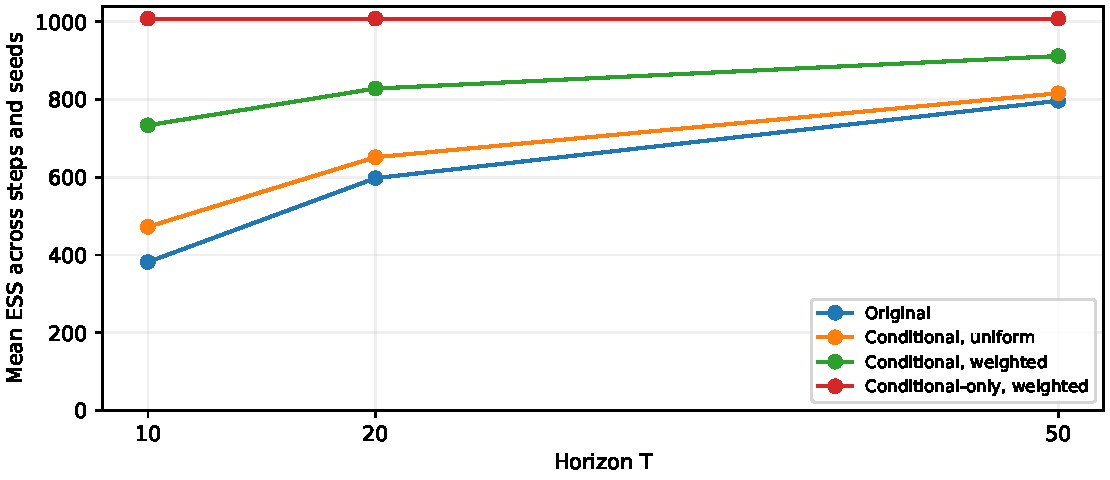
\includegraphics[width=.92\linewidth]{figures/observation-parent-nominal-ess.pdf}
\caption{Nominal-case ESS, averaged across time steps and eight streams.
The original, uniform conditional and weighted conditional mixtures have
mean ESS about $382$, $473$ and $734$ at $T=10$, respectively, and $797$,
$816$ and $912$ at $T=50$. The conditional-only weighted proposal has ESS
$1008$ up to roundoff. The rise with horizon includes later, easier observations;
it is not a claim that extending a filter inherently improves its weights.}
\label{fig:parent-nominal-ess}
\end{figure}

The ESS advantage extends beyond the nominal case. In each of the twenty
parameter--horizon cells with usable references, the weighted conditional
mixture has higher time-averaged ESS and higher minimum-over-time ESS than
the uniform conditional mixture in all eight paired streams: $160/160$
pairs for each measure. Averaging the time means over streams, the increase
ranges from $6.7\%$ to $102.7\%$ across those twenty cells. The same direction
holds in all $33$ parameter--horizon cells, or $264/264$ paired streams,
including cells whose Zhao--Cui references fail the accuracy checks. Comparing
ESS between the two proposals does not require those references. These are
descriptive comparisons of time means and minima; they do not establish that
ESS is higher at every individual time step or in future independent runs.

The comparison with uniform conditional parents isolates the additional
benefit, and cost, of parent weighting. Against both references, weighting
reduces log-likelihood RMSE in fifteen of the twenty usable cells, but
increases infection-score RMSE in thirteen, recovery-score RMSE in fifteen,
and noise-score RMSE in thirteen. Other cells favor weighting or have an
ordering that changes with the reference fit. Thus most of the score-error
reduction relative to the original is already present after conditioning
the children; redistributing children among parents does not produce a
uniform further score improvement.

Two noise-score comparisons meet the exploratory paired criterion. With
noise multiplier $0.8$ at $T=20$, weighting reduces RMSE from about $197.52$
to $12.34$--$12.35$. With noise multiplier $1.25$ at $T=50$, the direction
reverses: weighting gives $2.85$--$3.31$, compared with $1.08$--$1.10$ for
uniform parents. The first squared-error reduction has a $95\%$ interval
of approximately $[10183,67544]$ for either reference. In the second,
uniform parents reduce squared error by $6.95$ and $9.76$, with intervals
$[4.38,9.53]$ and $[6.84,12.69]$. Each sign-test value is $0.0078125$.
These are exploratory, cell-specific findings without multiplicity adjustment.

\begin{figure}[htbp]
\centering
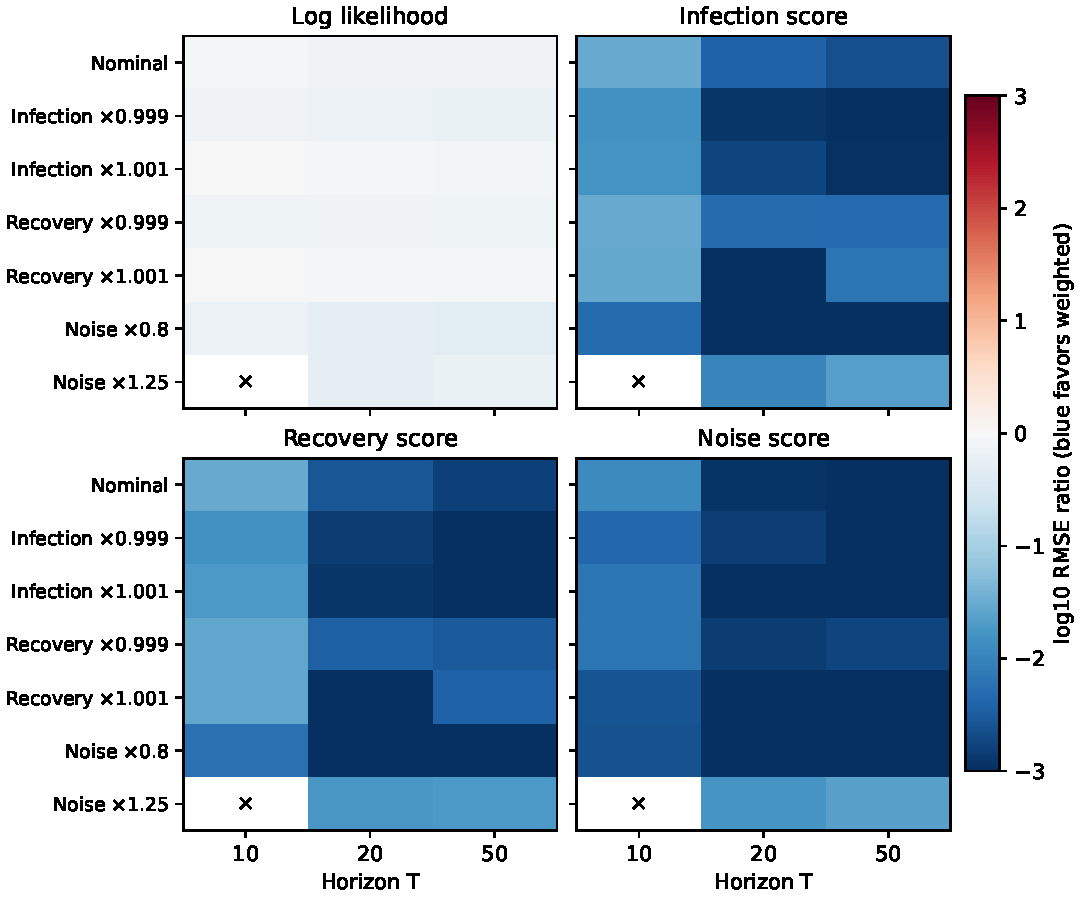
\includegraphics[width=\linewidth]{figures/observation-parent-accuracy-original.pdf}
\caption{Weighted conditional versus original proposal: observed RMSE ratios.
Color shows the mean across the two references of
$\log_{10}(\operatorname{RMSE}_{\rm weighted}/\operatorname{RMSE}_{\rm original})$.
Blue favors the weighted conditional mixture; color is saturated at $\pm3$.
A cross marks an unusable reference. None of these comparisons meets the full
exploratory paired MSE criterion. The twelve cells for rate multipliers
$0.9$ and $1.1$ are omitted because all fail reference overlap; their measured
values remain in the numerical record.}
\label{fig:parent-accuracy-original}
\end{figure}

\begin{figure}[htbp]
\centering
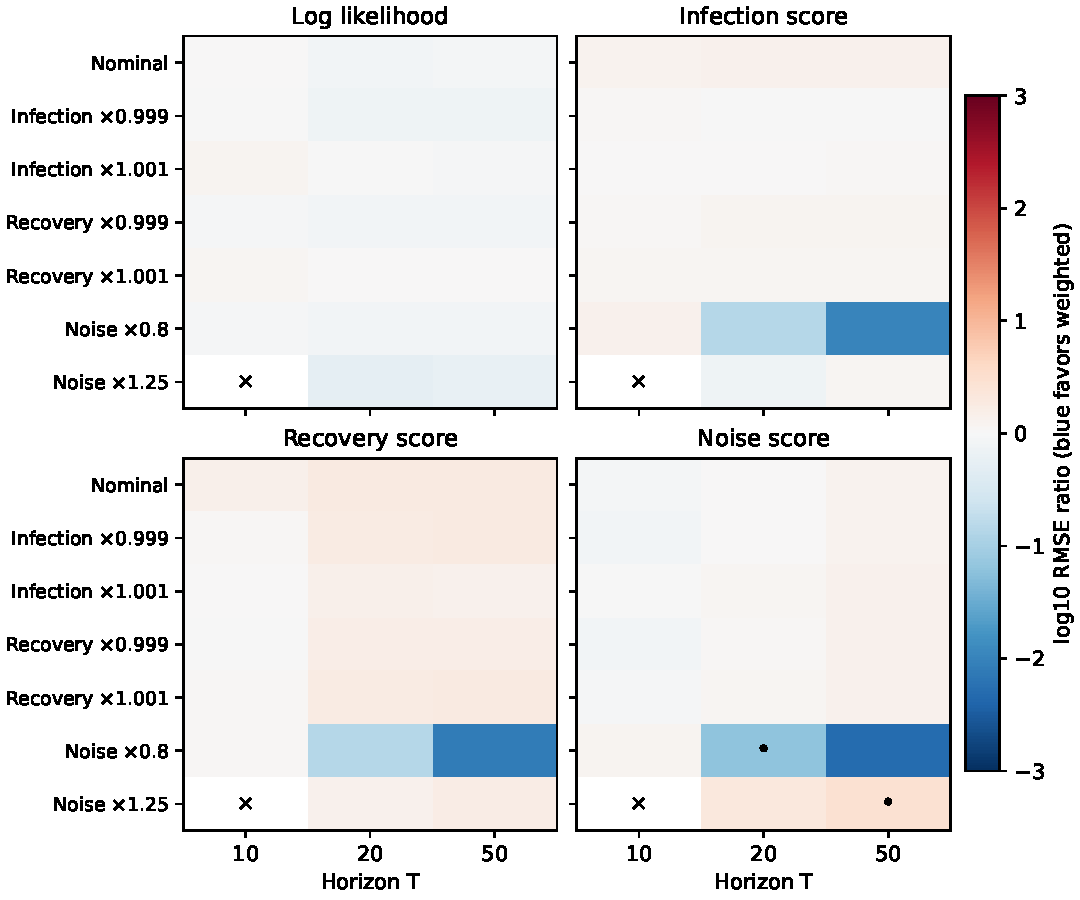
\includegraphics[width=\linewidth]{figures/observation-parent-accuracy-uniform.pdf}
\caption{Weighted versus uniform conditional parents: observed RMSE ratios,
with the same color scale and reference conventions as
Figure~\ref{fig:parent-accuracy-original}. A dot marks a comparison meeting the
exploratory paired criterion in the direction indicated by the color. The two
dots favor opposite parent-allocation rules, depending on noise and horizon.}
\label{fig:parent-accuracy-uniform}
\end{figure}

Simpler proposals expose a further limitation. At noise multiplier $1.25$,
$T=50$, the identity-only proposal has noise-score RMSE $1.16$--$1.21$ and
conditional-only uniform parents give $1.16$, both below the new mixture's
$2.85$--$3.31$. At nominal $T=50$, conditional-only weighted parents achieve
ESS $1008$ but infection-score RMSE $95.82$--$100.96$, compared with
$31.91$--$32.76$ for the conditional mixture with uniform parents. Equal
weights can coexist with a substantially less accurate score. These
conditional failures block a claim that the new mixture is accuracy-optimal,
even though the owner-selected default improves weight concentration.

Conditional and observation-weighted proposals remain the owner-selected
engineering default for their improved weight balance, with the uniform-parent
alternative retained for explicit comparisons. The accuracy comparison does
not establish that this default minimizes score error. It identifies the
remaining scientific work: larger rate changes need fresh, parameter-specific
Zhao--Cui fits; nominal and local comparisons need more paired streams to
resolve heavy-tailed squared-error uncertainty. Per-scope tuning, independent
datasets and the production precision require separate evaluation. The present
analytical scores are derivatives of a finite particle calculation with
categorical choices held locally fixed. Their agreement with local finite
differences establishes that derivative calculation, while their distance
from the approximate reference remains an empirical accuracy question.

The complete per-stream values, both-reference RMSEs, paired intervals,
conditional heuristic comparisons and reference vetoes are preserved in
\path{docs/plans/artifacts/observation-parent-sir-accuracy-20261028/analysis01/summary.json}
and its adjacent \path{tables.md}. The plan and result note record commands,
source hashes, numerical settings, review limitations and the compute budget.
